\documentclass{article}
\usepackage[utf8]{inputenc}
\usepackage[spanish]{babel}
\usepackage{listings}
\usepackage{subfigure}
\usepackage{graphicx}
\usepackage{url}
\usepackage{multirow}
\usepackage{color}
\usepackage{booktabs}
\usepackage{float}
\usepackage{amsmath}
\usepackage{verbatim}
\usepackage{hyperref}
\hypersetup{
    colorlinks=true,
    linkcolor=blue,
    filecolor=magenta,      
    urlcolor=cyan,
}
\usepackage[margin=3cm,twoside]{geometry} 
\setlength{\parindent}{0pt}
\setlength{\parskip}{1em}


\definecolor{mygreen}{rgb}{0,0.6,0}
\definecolor{mygray}{rgb}{0.5,0.5,0.5}
\definecolor{mymauve}{rgb}{0.58,0,0.82}
\lstset{ 
  backgroundcolor=\color{white},   % choose the background color; you must add \usepackage{color} or \usepackage{xcolor}; should come as last argument
  basicstyle=\footnotesize,        % the size of the fonts that are used for the code
  breakatwhitespace=false,         % sets if automatic breaks should only happen at whitespace
  breaklines=true,                 % sets automatic line breaking
  captionpos=b,                    % sets the caption-position to bottom
  commentstyle=\color{mygreen},    % comment style
  deletekeywords={...},            % if you want to delete keywords from the given language
  escapeinside={\%*}{)},          % if you want to add LaTeX within your code
  extendedchars=true,              % lets you use non-ASCII characters; for 8-bits encodings only, does not work with UTF-8
  firstnumber=1,                % start line enumeration with line 1000
  frame=single,	                   % adds a frame around the code
  keepspaces=true,                 % keeps spaces in text, useful for keeping indentation of code (possibly needs columns=flexible)
  keywordstyle=\color{blue},       % keyword style
  language=Octave,                 % the language of the code
  morekeywords={*,...},            % if you want to add more keywords to the set
  numbers=left,                    % where to put the line-numbers; possible values are (none, left, right)
  numbersep=5pt,                   % how far the line-numbers are from the code
  numberstyle=\tiny\color{mygray}, % the style that is used for the line-numbers
  rulecolor=\color{black},         % if not set, the frame-color may be changed on line-breaks within not-black text (e.g. comments (green here))
  showspaces=false,                % show spaces everywhere adding particular underscores; it overrides 'showstringspaces'
  showstringspaces=false,          % underline spaces within strings only
  showtabs=false,                  % show tabs within strings adding particular underscores
  stepnumber=1,                    % the step between two line-numbers. If it's 1, each line will be numbered
  stringstyle=\color{mymauve},     % string literal style
  tabsize=2,	                   % sets default tabsize to 2 spaces
  title=\lstname                  % show the filename of files included with \lstinputlisting; also try caption instead of title
}
\usepackage{etoolbox}
\makeatletter
\providecommand{\subtitle}[1]{% add subtitle to \maketitle
  \apptocmd{\@title}{\par {\large #1 \par}}{}{}
}
\renewcommand{\theenumi}{\roman{enumi}}
\newtheorem{teor}{Teorema}
\makeatother
\title{Tarea 7 de Modelos Probabilistas Aplicados}
\subtitle{Transformaciones mediante Escalera de poderes de Tukey }

\author{5271}
\date{\today}

\begin{document}

\maketitle

\section{Introducción}

En este trabajo se realiza un breve acercamiento al tema Transformaciones mediante Escalera de poderes de Tukey y regresión lineal. Además presenta un algoritmo desarrollado en lenguaje R para extraer la función que genera la variable dependiente así como sus coeficientes. La experimentación se realiza en el programa R versión 4.0.2 \cite{r} en el entorno de desarrollo Rstudio \cite{rstudio}

\section{Transformaciones mediante Escalera de poderes de Tukey}

Para entender mejor como funciona las transformaciones mediante Escalera de poderes de Tukey creamos un \textit{data.frame} con datos bivariados $(x_{1} , y)$ de manera que $x_{1}$ se distribuye uniformemente e $y = ax_{1}+b$. Lo anterior se realiza con el código \ref{cod:1} en R. 
\begin{center}
\lstinputlisting[ language=R, firstline=1, lastline=6]{Tarea7n.R}
\label{cod:1}
\end{center}

Como primer paso se trazan los datos en un diagrama de dispersión. En la figura \ref{fig:1} de la página \pageref{fig:1} se puede observar como se relaciona las variables $x_{1}$ e $y$. Como se aprecia en dicha figura la relación entre $x_{1}$ e $y$ es una dependencia lineal y si aplicamos una regresión lineal obtendremos exactamente los coeficientes y formulación con la cual se crea la variable dependiente $y$. A continuación se metra el resultado de aplicar la regresión lineal. De donde se pueden extraer los coeficientes $a$ y $b$ de la ecuación, quedando $y = 15x_{1}+8$.  

\verbatiminput{txt/lm1.txt}

\begin{figure}
\centering
\subfigure[$y = ax_{1}+b$]{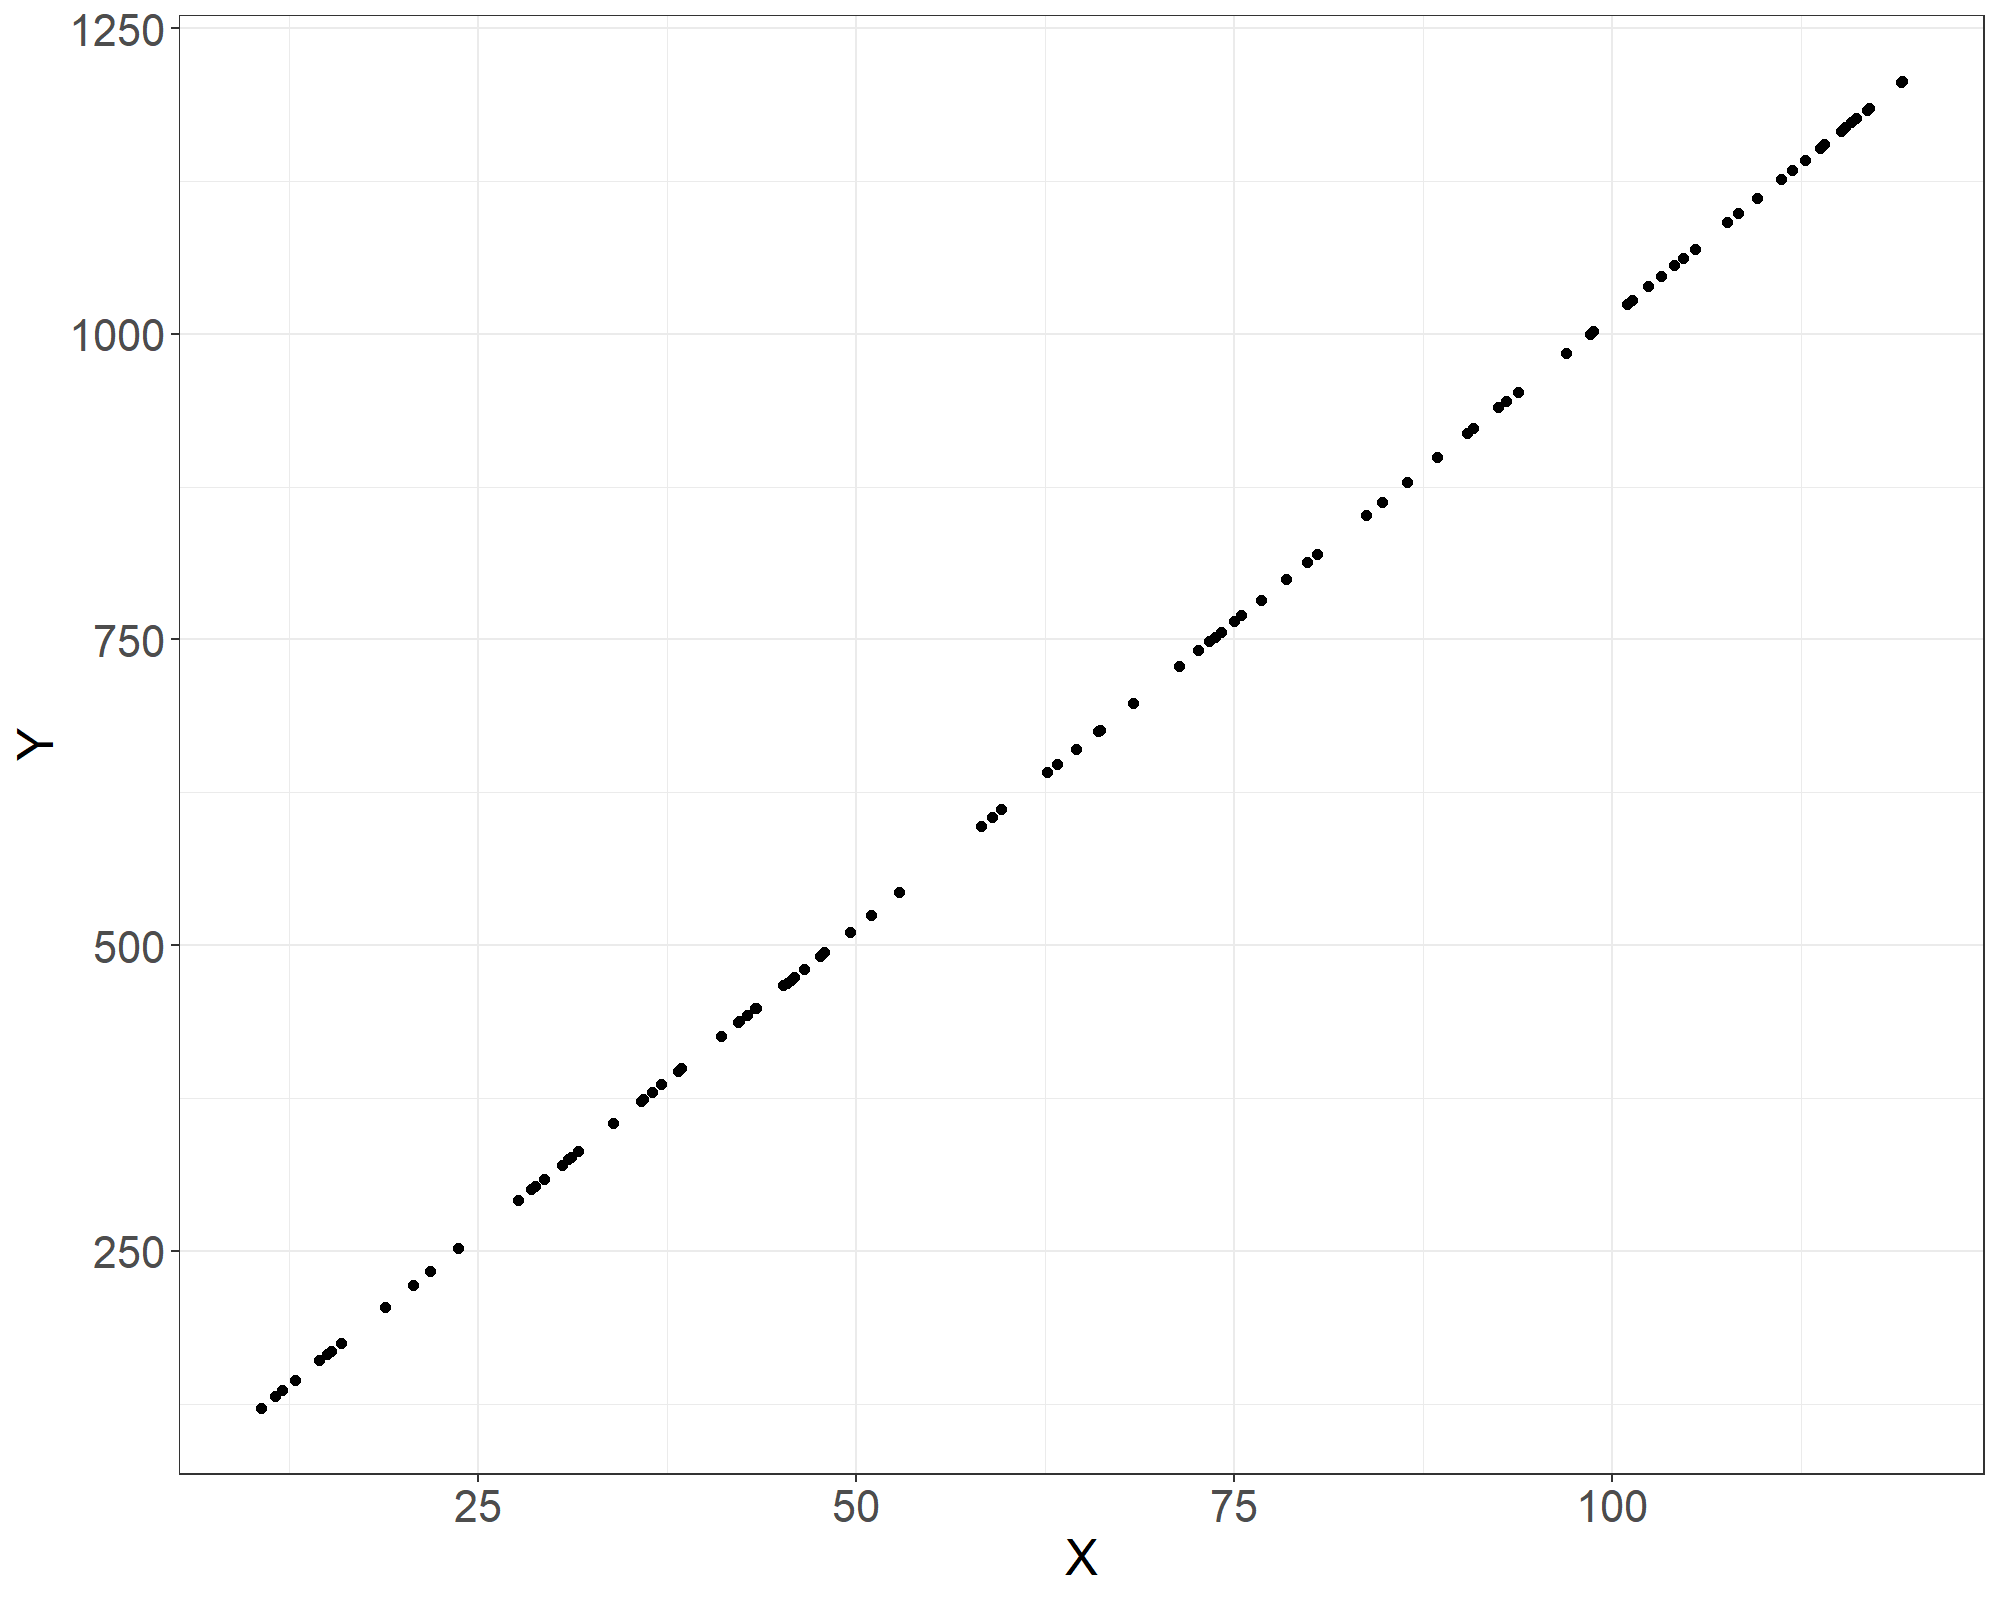
\includegraphics[scale=0.30]{figuras/recta.png}}
\label{fig:a}
\centering
\subfigure[regresión lineal]{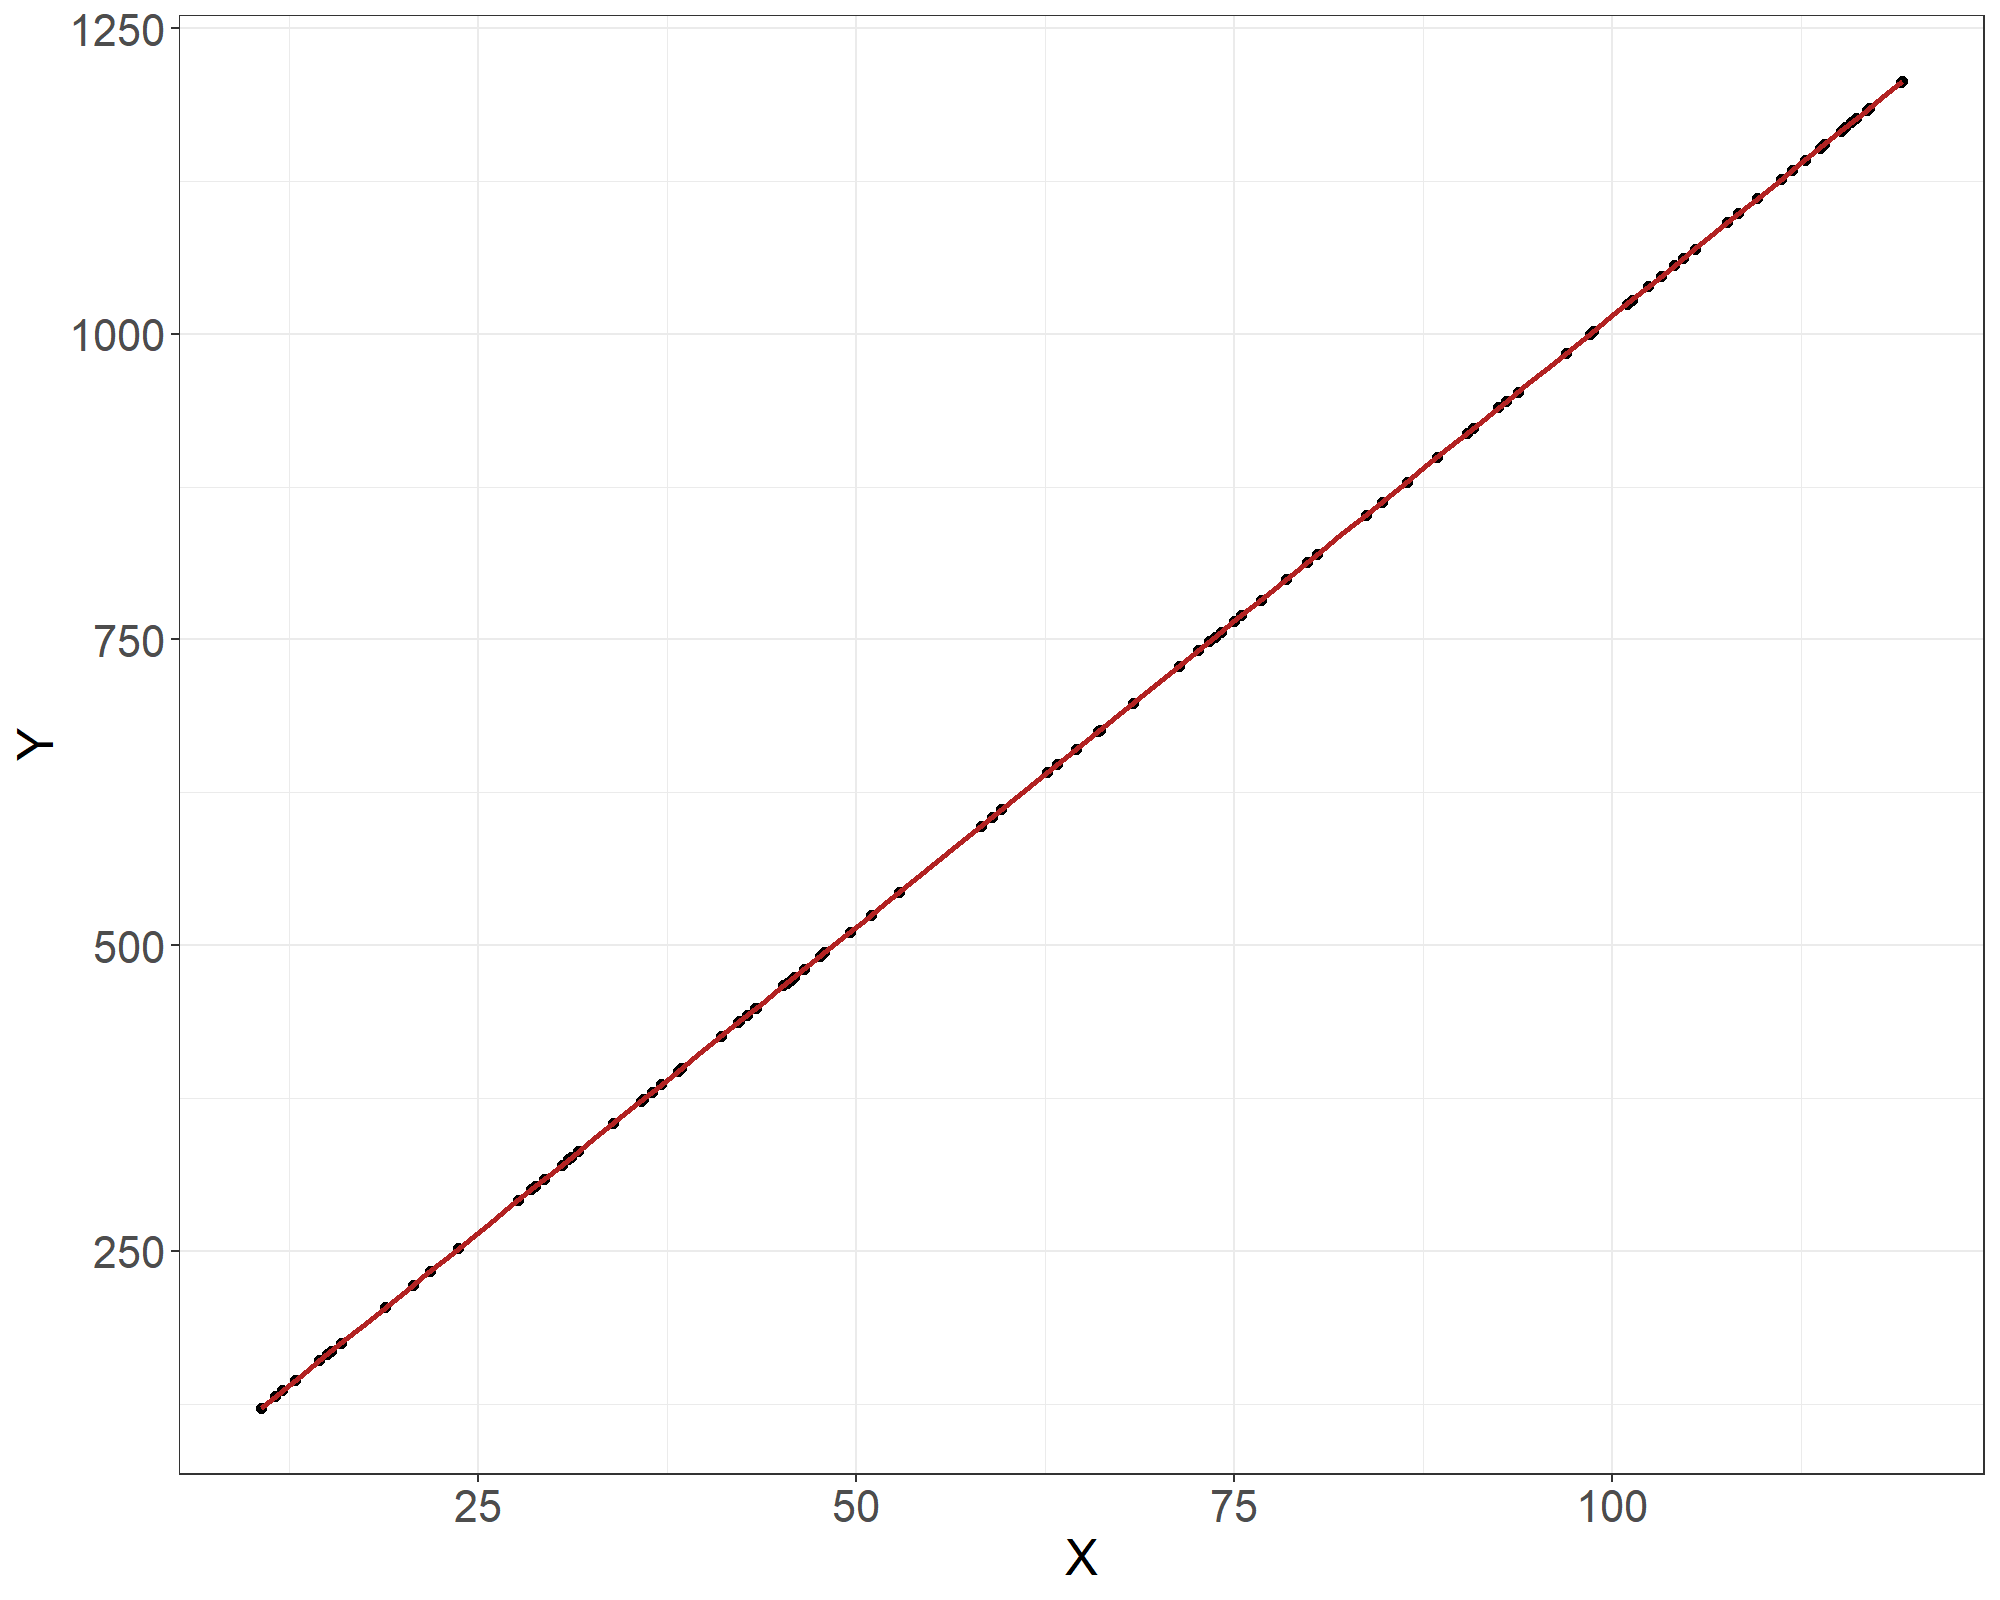
\includegraphics[scale=0.30]{figuras/rectar.png}}
\label{fig:b}
\centering
\caption{Diagramas de dispersión de los datos bivariados $(x_1 , y)$ }
\label{fig:1} 
\end{figure}
El ejemplo anterior es sencillo pues con solo una regresión lineal se pueden obtener los coeficientes y la función que crea a $y$. En cambio si creamos representamos los datos bivariados creados con $y= a*log(x_1)+ b$, se puede observar en la figura \ref{fig:2} de la página \pageref{fig:2} que la relación de dependencia no es lineal, por lo que una simple regresión no arrogará los resultados deseados, por lo cual antes de aplicar la regresión se debe hacer una transformación a una de las variable, es decir tratar de linealizar la relación de dependencia.

No hay ninguna restricción sobre los valores de $\lambda$ que podamos considerar. Obviamente, elegir $\lambda = 1$ deja los datos sin cambios. Los valores negativos de $\lambda$ también son razonables. Lo que da lugar a la ecuación \ref{eq:2}. El cuadro \ref{tab:2} de la página \pageref{tab:2} se muestran ejemplos de la escalera de transformaciones de Tukey.

Tukey sugiere explorar relaciones como:
\begin{equation}\label{eq:1}
y=ax_{1}^{\lambda}+ b    
\end{equation}
donde $\lambda$ es una parámetro que elegido con el fin de linealizar la relación. 

\begin{equation}\label{eq:2}
y= \left\lbrace 
\begin{array}{lr}
\textup{$x^{\lambda}$}\quad \quad\:\: \text{si} \lambda >0 \\
\textup{log x} \quad \:\: \text{si} \lambda = 0 \\
\textup{$-(x^{\lambda})$}\quad \text{si} \lambda <0 \\
\end{array}
\right.
\end{equation}

\begin{table}[]\caption{Escalera de transformaciones de Tukey}
\centering
\begin{tabular}{| l | c | c | c | c | c | c | c |}
\hline
$\lambda$ & -2&  -1& -1/2 & 0  &1/2 & 1 & 2\\
\hline 
\texttt{y} & $\frac{-1}{x^2}$ & $\frac{-1}{x}$ &  $\frac{-1}{\sqrt{x}}$ & $\log x$ & $\sqrt{x}$ & $x$ & $x^2$\\
\hline 
\end{tabular}
\label{tab:2}
\end{table}

\begin{figure}
\centering
\subfigure[$y = a*log(x_{1})+b$]{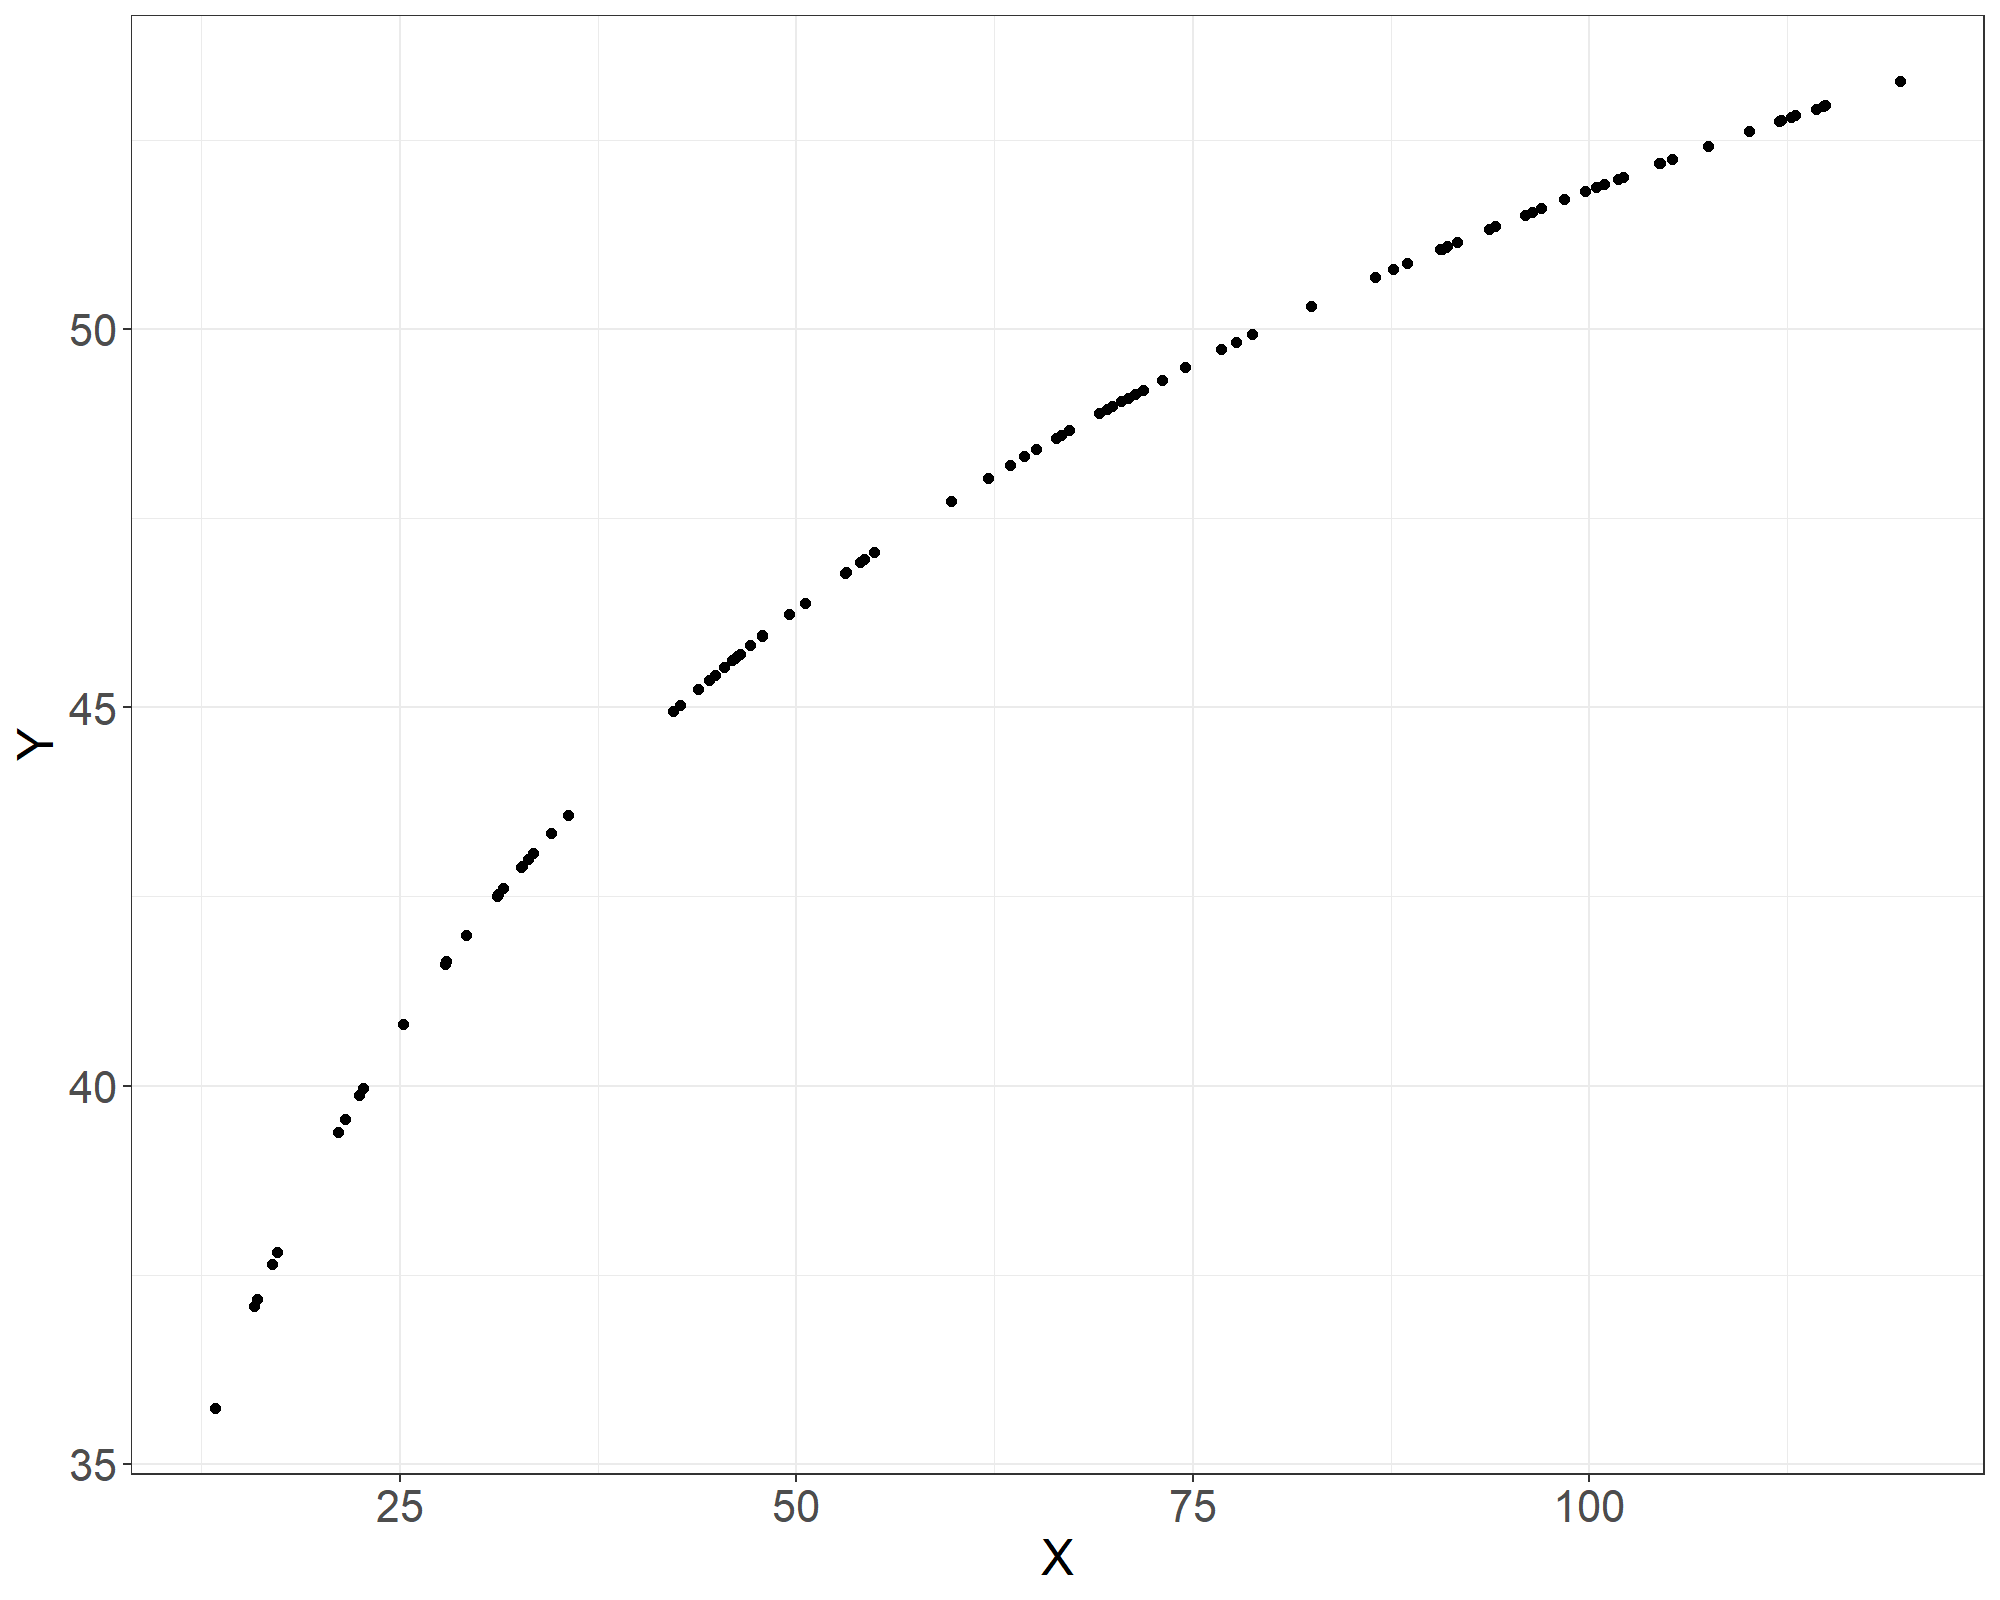
\includegraphics[scale=0.30]{figuras/log.png}}
\label{fig:a}
\centering
\subfigure[regresión lineal]{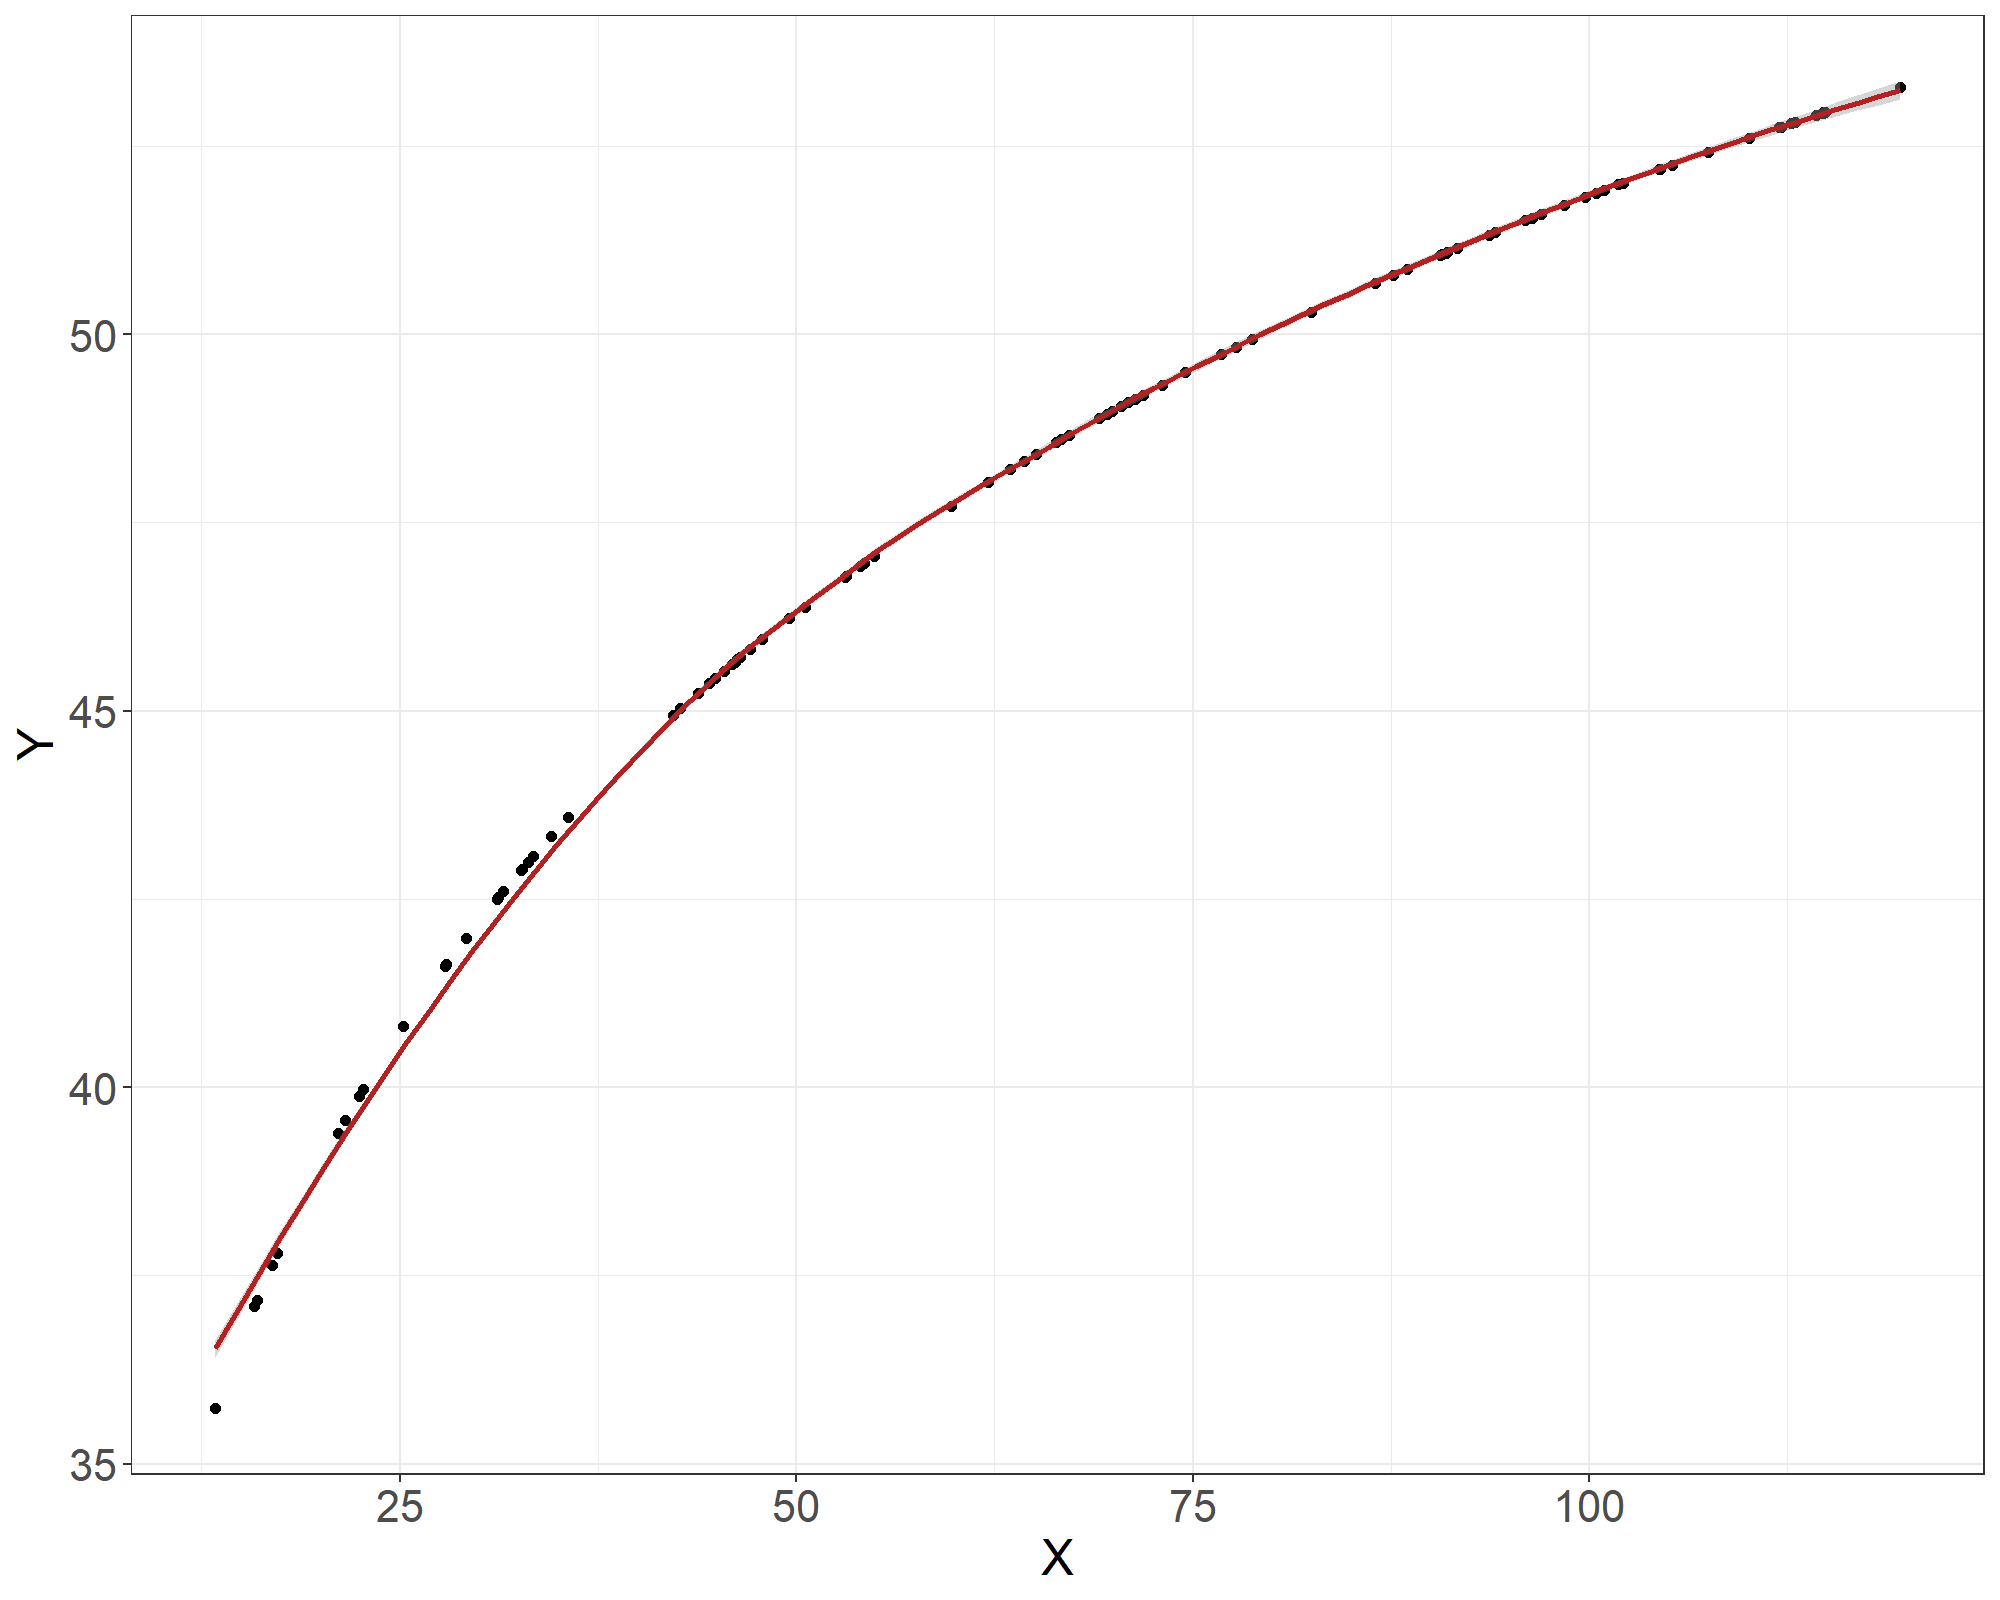
\includegraphics[scale=0.30]{figuras/logr.png}}
\label{fig:b}
\centering
\caption{Diagramas de dispersión de los datos bivariados $(x_1 , y)$ con dependencia no lineal}
\label{fig:2} 
\end{figure}

Se Aplica transformaciones mediante la escalera de Tukey a los datos, en forma que se calcula el logaritmo de la variable $x_{1}$, y se vuelve a representar los datos y se realiza la regresión lineal. En la figura \ref{fig:3} de la página \pageref{fig:3} se puede observar la transformación de los datos.

\begin{figure}
\centering
\subfigure[$y = a*log(x_{1})+b$]{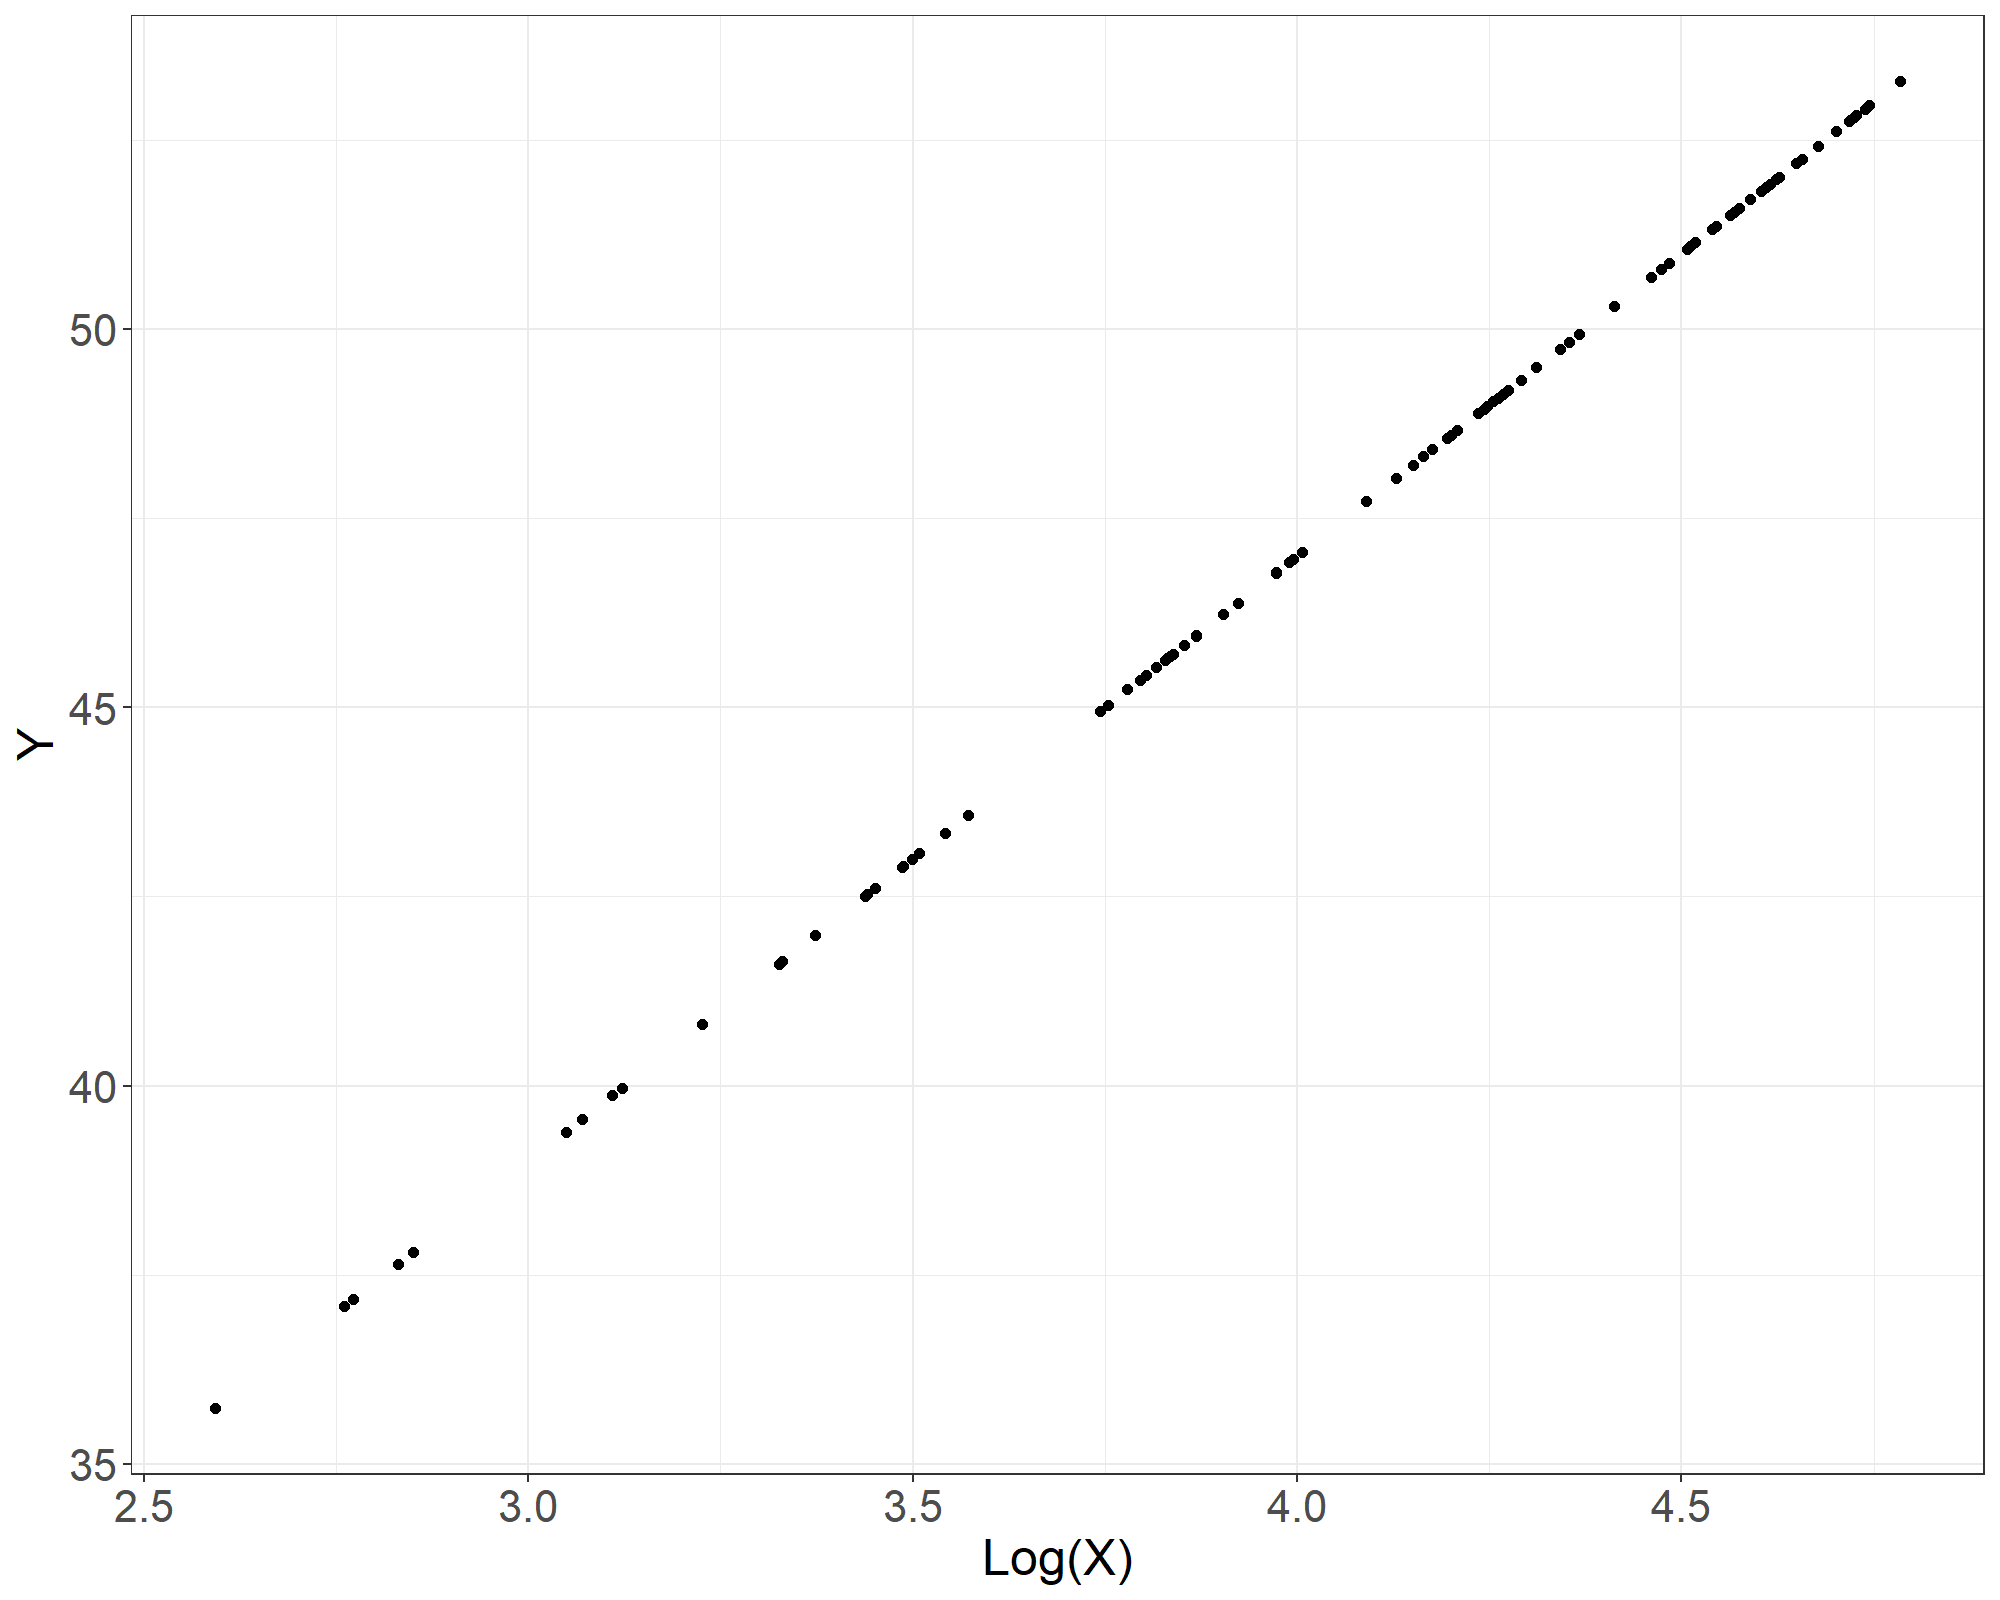
\includegraphics[scale=0.30]{figuras/logt.png}}
\label{fig:a}
\centering
\subfigure[regresión lineal]{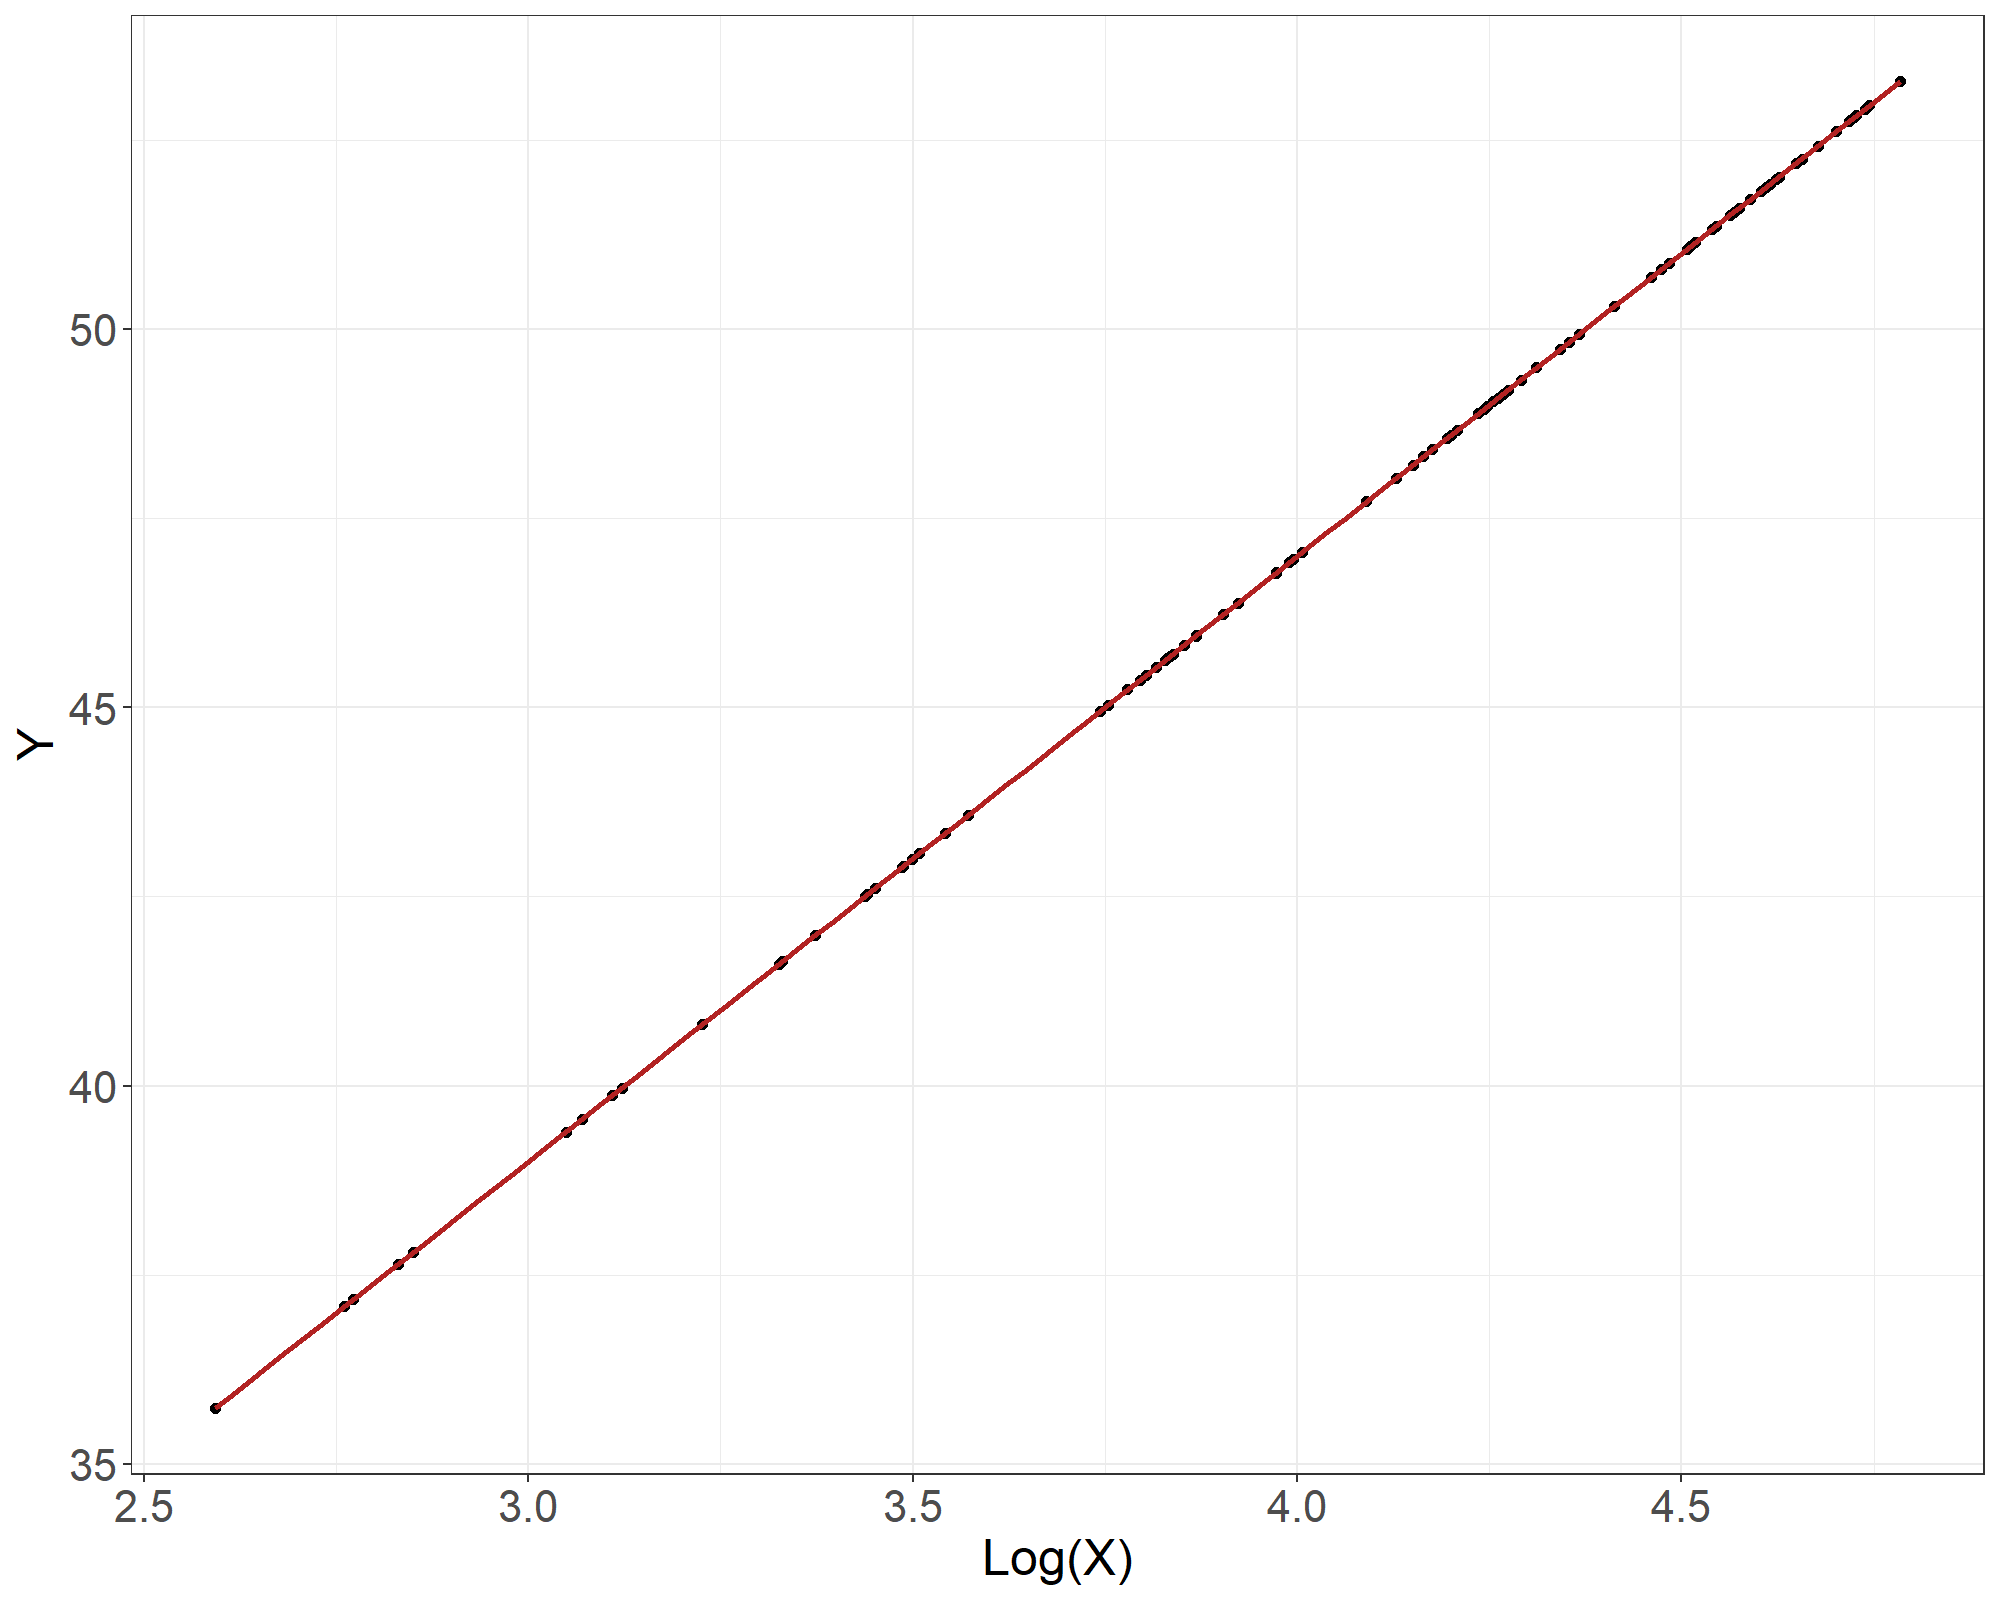
\includegraphics[scale=0.30]{figuras/logrt.png}}
\label{fig:b}
\centering
\caption{Diagramas de dispersión de los datos bivariados $(x_1 , y)$ con dependencia no lineal}
\label{fig:3} 
\end{figure}
\section{Algoritmo propuesto}

Según lo visto en la sección anterior podemos mediante las transformaciones de la Escalera de Tukey, podemos acercar la relación entre los datos bivariados a una dependencia lineal. A partir de está conclusión se creo una función en R que la pasarle como parámetros un \textit{data.frame} y la cantidad de variables de cuales depende $y$ (máximo tres variables), devuelve un \textit{data.frame} con los valores de $\lambda$ encontrados para la linealización, los coeficientes de la función y el error estándar de la estimación delos coeficientes. En el código \ref{cod:2} se muestra dicha función. 
\begin{center}
\lstinputlisting[ language=R, firstline=8, lastline=128]{Tarea7n.R}
\label{cod:2}
\end{center}
\section{Resultados}
En el cuadro \ref{fig:3} de la página \pageref{fig:3} se observan los resultados obtenido para diferentes funciones.



El código general se encuentra disponible en el repositorio. \href{https://github.com/Albertomnoa/Tareas_MPA/tree/master/Tarea4}{https://github.com/Albertomnoa/Tareas} 

\newpage
\bibliographystyle{plain}
\bibliography{Biblio}

\end{document}
